\chapter{Recalibrating the archive products (improved v1)}
\label{sec:app_v1}
Before \banzai{} was run from the raw frames, the corrections were developed on the public \texttt{-1d}/\texttt{-2d}
products of \banzai{}~1.0.1. Those products had already been divided by a shifted lamp flat, so the division had to
be undone, the destroyed pixels masked, and the sky and the extraction redone before the fringe model could be applied.
This appendix documents that procedure (improved v1, Table~\ref{tab:versions_names}). It is not part of the pipeline
run from raw (improved v2 and v3), which never divides by a flat and uses \banzai's own sky model and extraction; it
remains useful for reprocessing archive products for which the raw frames are not available
(\texttt{banzai\_floyds.diagnostics.reextract}, Chapter~\ref{sec:software}).

\section{Undoing the division and the master pattern}
\label{sec:fringe_master}
The frame before the division is recovered as
\begin{equation}
R(x,y)=\begin{cases} I(x,y)\,\Phi(x,y) & 0.5<\Phi<2\\ I(x,y) & |\Phi|<10^{-3}\ \text{(not applied)}\\
\text{masked} & \text{otherwise,}\end{cases}
\label{eq:undo}
\end{equation}
with $I$ the \texttt{SCI} image, and likewise for the uncertainty. Each frame's map is the lamp pattern
$\Pi$ shifted along the slit, $\Phi_f(x,y)=\Pi(x,y-o_f)$, so $\Pi$ is recovered by shifting $\Phi_f$ by $-o_f$
(linear interpolation; pixels with interpolation weight $<0.99$ discarded). The 61 maps with $|o_f|<40$ give
patterns that agree with their median $\bar\Pi$ with $r=0.998$--1.000. The fringe component is
\begin{equation}
\delta(x,y) = w(\lambda)\left[\frac{\bar\Pi(x,y)}{\mathcal{M}_{41}[\bar\Pi](x,y)}-1\right],\qquad
w(\lambda)=\min\!\left[\max\!\left(\frac{\lambda-6500}{300},0\right),1\right],
\label{eq:delta}
\end{equation}
where $\mathcal{M}_{41}$ is a running median of 41 pixels along the dispersion. This removes the slit-illumination
bands and the smooth flat structure and keeps the fringes (period $\approx11$\,pixels along the dispersion,
10.9 per cent rms at 7000--9500\,\AA; Fig.~\ref{fig:master}).

\begin{figure}[!htbp]
\centering
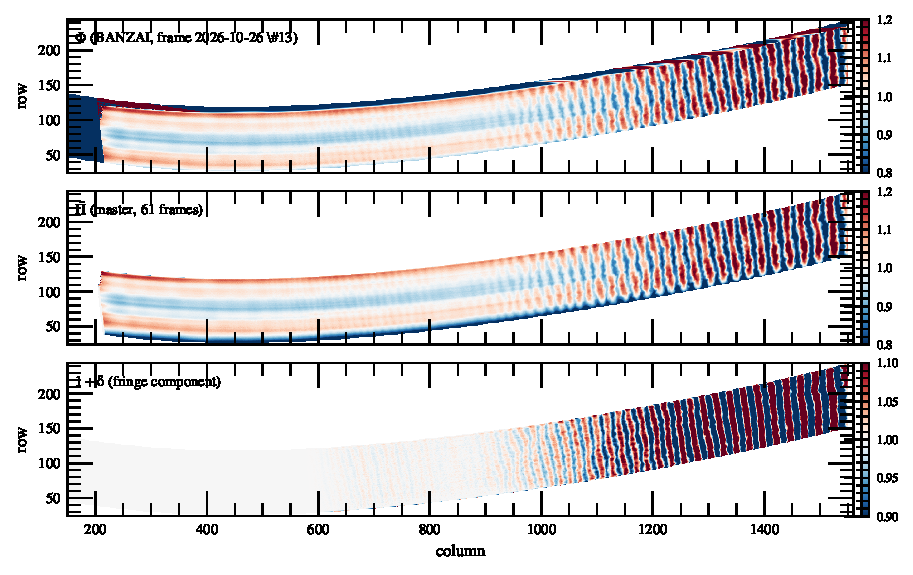
\includegraphics[width=\textwidth]{figures/fig_master.pdf}
\caption{Red order. Top: the map $\Phi$ the archive frame 2026-10-26 \#13 was divided by (shifted by $-8.9$ rows; note
the invalid edges). Middle: the master lamp pattern $\bar\Pi$ from the un-shifted maps of 61 frames. Bottom: its fringe
component $1+\delta$ (eq.~\ref{eq:delta}).}
\label{fig:master}
\end{figure}

\section{Fringe fit}
\label{sec:fringe_fit}
\textit{Shift.} To first order $R=R_0(1+a\,\delta)$ with $R_0$ smooth along the dispersion on fringe scales. With
$\mathcal{H}[\cdot]$ the residual from a 21-pixel running median along $x$, for every trial shift $(\Delta x,\Delta y)$
on a 0.5-pixel grid with $|\Delta x|,|\Delta y|\le2$,
\begin{equation}
\hat a=\frac{\sum w\,\mathcal{H}[R]\,\mathcal{H}[R\,\delta']}{\sum w\,\mathcal{H}[R\,\delta']^2},\qquad
\chi^2(\Delta x,\Delta y)=\sum w\left(\mathcal{H}[R]-\hat a\,\mathcal{H}[R\,\delta']\right)^2,
\label{eq:fringe2d}
\end{equation}
where $\delta'(x,y)=\delta(x-\Delta x,y-\Delta y)$, $w=1/\sigma_R^2$, and the sums run over the red-order pixels at
7000--9800\,\AA{} more than 6 rows from the slit ends. The minimum is well defined (period $\approx11$\,pixels in
$\Delta x$) and lies at $|\Delta x|\le1$, $|\Delta y|\le1$ for all frames.

\textit{Amplitude (initial model).} The 2-d fit under-corrects, so the correction is applied to the extracted spectrum. The profile-weighted fringe of each 1-pixel bin $\beta$ is
\begin{equation}
f_\beta=\frac{\sum_{i\in\beta}P_i\,\delta'_i}{\sum_{i\in\beta}P_i},
\label{eq:fringe1d}
\end{equation}
and the extracted counts are divided by $1+A(\lambda)f_\beta$, where the shift of $\delta'$ is the 2-d one.
The amplitude $A(\lambda)$ can be fitted freely on a spectrum by linear least squares of
$\mathcal{H}_{\rm 1d}[F]$ on $\mathcal{H}_{\rm 1d}[F\,f]$ ($\mathcal{H}_{\rm 1d}$: difference of 25\,\AA{} and 200\,\AA{}
running medians, telluric bands excluded) in a wavelength region. This is reliable on the smooth standards but not on
a single AGN spectrum, where it latches onto real structure. The amplitude is, however, very stable within one
instrument configuration, so it is calibrated per slit width as the median of the free fits over an ensemble of
frames, in four regions (6800--7500, 7500--8300, 8300--9100, 9100--9800\,\AA), and interpolated linearly between their
centres (Table~\ref{tab:amplaw}). Regions where the median is negative or its scatter exceeds half its value
(6800--7500\,\AA, where $\delta$ is still tapered in and most pixels are telluric) take the value of the nearest
reliable region. This uses no target information. The amplitude exceeds unity because the stored lamp map has a
diluted fringe contrast, and it differs between the 2 and 6\,arcsec slits, plausibly because slit-filling light reaches
each pixel over a wider wavelength range in a wide slit. This model is kept as an option
(\texttt{method='amplitude'}); Section~\ref{sec:fringe_harmonic} explains why it leaves $\approx5$ per cent
residuals and describes the default model.

\begin{table}
\centering
\caption{Fringe amplitude $A(\lambda)$ per slit width: median and robust scatter of the free fits over the ensemble of frames. $^{a}$Unreliable region (negative or scatter $>$ half the value); the value of the nearest reliable region is used.}
\label{tab:amplaw}
\begin{tabular}{lcccc}
\toprule
Slit & 7150\,\AA & 7900\,\AA & 8700\,\AA & 9450\,\AA \\
 & \multicolumn{4}{c}{($A$, no unit: multiplies the normalised fringe pattern)} \\
\midrule
6\,arcsec (50 frames) & \AmpSixA & \AmpSixB & \AmpSixC & \AmpSixD \\
2\,arcsec (18 frames) & \AmpTwoA & \AmpTwoB & \AmpTwoC & \AmpTwoD \\
\bottomrule
\end{tabular}
\end{table}



\section{Sky model}
\label{sec:sky}
For every 1-pixel wavelength bin $\beta$ of an order (\banzai{}'s binning, which follows the line tilt), the sky is a
polynomial along the slit,
\begin{equation}
S_\beta(y_{\rm o})=\sum_{k=0}^{2}b_{\beta k}\,y_{\rm o}^k,
\label{eq:sky}
\end{equation}
fitted by weighted least squares to the unmasked pixels with $|y_{\rm p}|>m\,\sigma_{\rm p}$ and
$|y_{\rm o}|<y_{\rm max}-6$, with iterative $3\sigma$ clipping. The mask half-width is $m=4$ unless that leaves fewer
than 25 per cent of the slit's pixels, in which case $m$ is reduced to the corresponding quantile of
$|y_{\rm p}|/\sigma_{\rm p}$ (but not below 2); the degree is reduced while fewer than $4(K+1)$ sky pixels remain, and set
to zero when all sky pixels lie on one side of the object. When the mask has been reduced, the sky pixels contain the
object's wings, so the sky polynomial and the object are fitted jointly to all slit pixels,
$R_i=\sum_k b_{\beta k}y_{{\rm o},i}^k+F'_\beta P_i$, with iterative clipping; only the sky part is kept. In synthetic
tests with $\sigma_{\rm p}=9$\,pixels in a 60-row slit this removes an 11 per cent flux bias. Its covariance
$C_\beta=(V^{\rm T}WV)^{-1}$ ($V$ the Vandermonde matrix, $W$ the inverse variances) is propagated into the
extraction errors. This replaces the 2-d spline sky of \banzai{} \citep{Kelson2003}, which cannot follow the
discontinuities introduced by the fringe map.

\section{Extraction}
\label{sec:extraction}
For bin $\beta$, with net counts $d_i=R_i-S_\beta(y_{{\rm o},i})$, profile weights $P_i$ (\banzai's fitted profile,
normalised to unit sum per column) and pixels within $|y_{\rm p}|<5\sigma_{\rm p}$, the optimal extraction
\citep{Horne1986} is
\begin{equation}
F_\beta=\frac{\sum_i a_i d_i}{\sum_i a_i P_i},\qquad a_i=\frac{P_i}{V_i},\qquad
V_i = r^2+\max(F_\beta P_i+S_{\beta,i},0),
\label{eq:horne}
\end{equation}
iterated with $V$ from the model (not the data); at each iteration the single pixel with the largest
$(d_i-F_\beta P_i)^2/V_i$ is rejected if this exceeds 25 (cosmic rays), up to $\max(2,\,0.1N_\beta)$ pixels per bin
(more ``outliers'' indicate a profile mismatch, not cosmic rays). The read noise is $r=3.5\,e^-$. Its variance is
\begin{equation}
\sigma^2_{F_\beta}=\frac{\sum_i a_i^2V_i+\mathbf{g}^{\rm T}C_\beta\,\mathbf{g}}{\left(\sum_i a_iP_i\right)^2},\qquad
\mathbf{g}=\sum_i a_i\,\mathbf{v}_i,
\label{eq:hornevar}
\end{equation}
with $\mathbf{v}_i=(y_{{\rm o},i}^2,y_{{\rm o},i},1)$ the sky basis at pixel $i$. A fixed-aperture extraction for RM is
\begin{equation}
F^{\rm box}_\beta=\frac{\sum_{|y_{\rm p}|<h}d_i}{\sum_{\rm all\ rows}P_i},
\label{eq:boxcarext}
\end{equation}
with $h=10$\,pixels ($\pm3.4$\,arcsec) by default; the denominator is the number of columns the bin spans, which
gives the same normalisation as \banzai{} for bins that collect 0, 1 or 2 pixels per row. In synthetic tests the
recovered fluxes are unbiased (optimal 2 per cent, boxcar 3 per cent including a cosmic ray on the trace) and the
normalised residuals have rms 1.03 (optimal) and 1.09 (boxcar).

\section{Results}
\label{sec:results_fringe}
Fig.~\ref{fig:edge} shows the frame region where the shifted lamp flat had destroyed the data; the stripes are gone
and the largest number of spikes in a spectrum drops from \SpMaxOld{} to \SpMaxNew. Fig.~\ref{fig:residuals} shows the
2-d residuals: in the bright-moon frame the robust rms of the normalised residuals at 7000--9500\,\AA{} drops from
1.70 to 1.44 in the sky rows and from 1.83 to 1.41 on the object; on the standard from 1.17 to 1.09 and 1.98 to 1.90.
In the dark frame the residuals are dominated by a mismatch of the (common) profile model and are unchanged (1.12 and
1.14 in the sky rows). Fig.~\ref{fig:fringe1d} compares extracted red orders. The fringe metric of the Fairall~9 spectra
drops from \FrOld{} to \FrNewOpt{} per cent and the fringing in the median spectrum from \FrMedOld{} to \FrMedNewOpt{}
per cent (Fig.~\ref{fig:series}); on the EG\,21 spectra from \EGfrOld{} to \EGfrNew{} per cent. This metric
smooths over 25\,\AA{} and includes real spectral structure and telluric residuals in its windows; the unsmoothed
comparison of Table~\ref{tab:fringevariants} isolates the fringe correction: the harmonic model halves the residual
of the amplitude law and comes within a factor $\approx2$ of the photon-noise floor (Fig.~\ref{fig:harmonic}). Because RM fits every
spectrum separately, Fig.~\ref{fig:individual} shows all spectra individually, divided by a power law: in the archive
products every spectrum carries 10--20 per cent fringes; after the correction the residual in the clean windows is
\IndivNewF{} per cent for Fairall~9 and \IndivNewE{} per cent for EG\,21 (\banzai: \IndivOldF{} and \IndivOldE), and no
periodic pattern is left in single spectra; the faintest spectra (signal-to-noise ratio 11--16 per pixel, 3--4\,arcsec
seeing) are photon-noise limited. The individual spectra also expose a feature that is \emph{not} a fringe residual:
a step of $\approx30$ per cent at $\approx9285$\,\AA{}, preceded by a bump in the gap between water bands at
9240--9285\,\AA, present in every version including the first one. Redward of 8900\,\AA{} there is no telluric-free
continuum: both the continuum used to measure the telluric transmission and the sensitivity correction are extrapolated
from shorter wavelengths, and the transmission is clipped to unity in the gap. The red end beyond 8900\,\AA{} is
therefore not yet reliably flux-calibrated (Chapter~\ref{sec:recommendations}). The residual in the A band also grows
with the width of the object's profile (Spearman $\rho=0.80$; 4 per cent for FWHM $<2.5$\,arcsec against 9 per cent
above, photon noise removed), because the telluric transmission measured on the 2\,arcsec standards is not matched to
the line-spread function of the 6\,arcsec spectra, which the seeing sets.

\begin{figure}[!htbp]
\centering
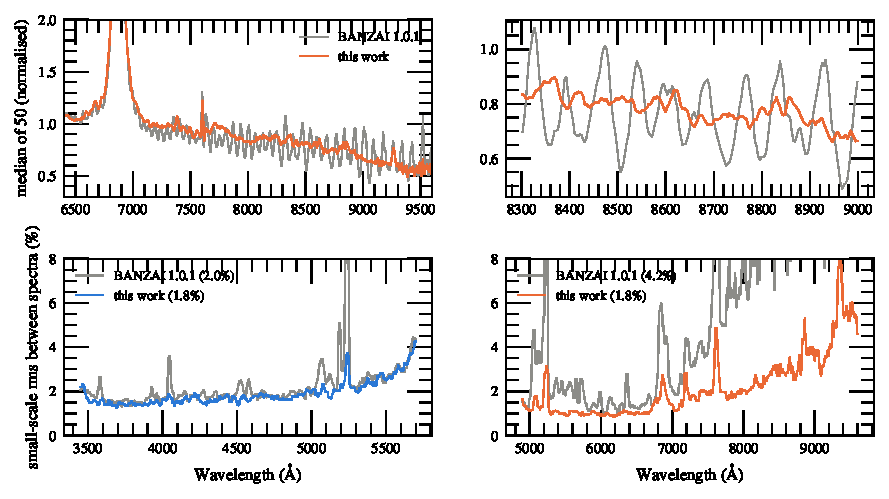
\includegraphics[width=\textwidth]{figures/fig_series.pdf}
\caption{Fairall~9, 50 spectra. Top: median red-order spectrum (left) and a zoom (right). Bottom: small-scale
($<200$\,\AA) scatter between the spectra, blue (left) and red (right) orders; archive in grey.}
\label{fig:series}
\end{figure}


\begin{figure}[!htbp]
\centering
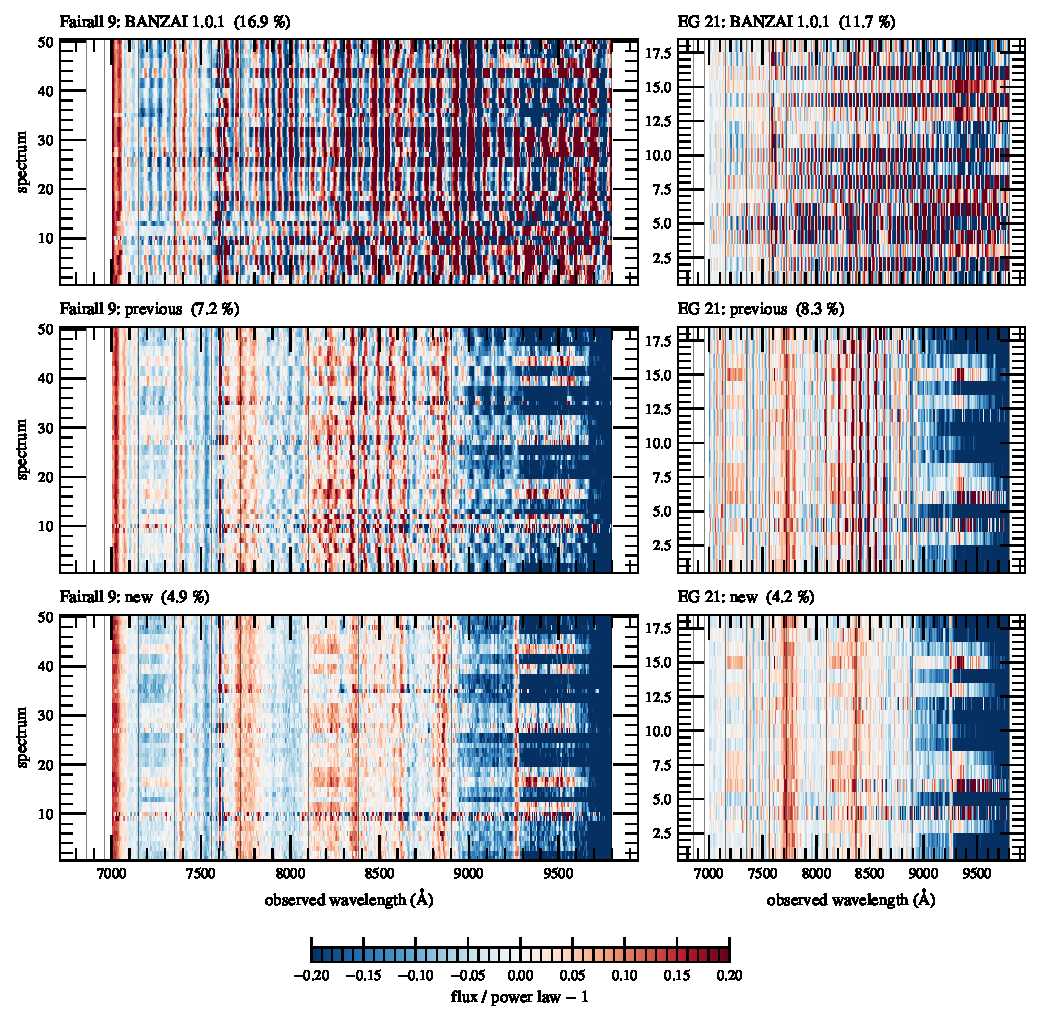
\includegraphics[width=\textwidth]{figures/fig_individual.pdf}
\caption{Individual flux-calibrated red-order spectra (one row per spectrum, in time order) divided by a power law
fitted at 7000--9800\,\AA{} outside the telluric bands (marked by vertical lines). Left: the 50 Fairall~9 spectra;
right: the 18 EG\,21 spectra. Top: \banzai{}~1.0.1; middle: initial model of the correction (lamp pattern times
amplitude law); bottom: this work (harmonic model, two passes). The number in each title is the median over spectra of
the rms in 7750--8050 and 8450--8900\,\AA. Remaining vertical structure is common to all spectra (broad lines of
Fairall~9, telluric residuals); horizontal bands beyond 9300\,\AA{} are night-to-night changes of the water-vapour
absorption.}
\label{fig:individual}
\end{figure}


\begin{figure}[!htbp]
\centering
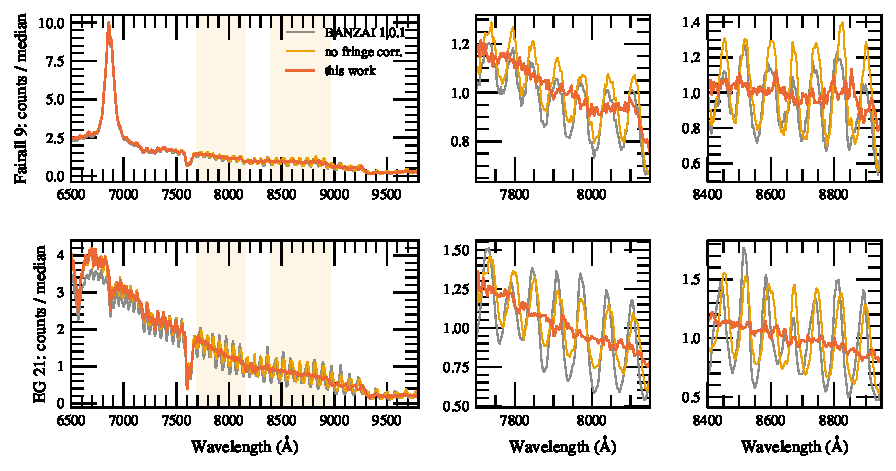
\includegraphics[width=\textwidth]{figures/fig_fringe1d.pdf}
\caption{Extracted red order (counts, normalised) of a Fairall~9 frame and an EG\,21 frame: archive (grey), fringe
division undone without new correction (yellow), this work (orange). The zooms are free of telluric bands.}
\label{fig:fringe1d}
\end{figure}


\begin{figure}[!htbp]
\centering
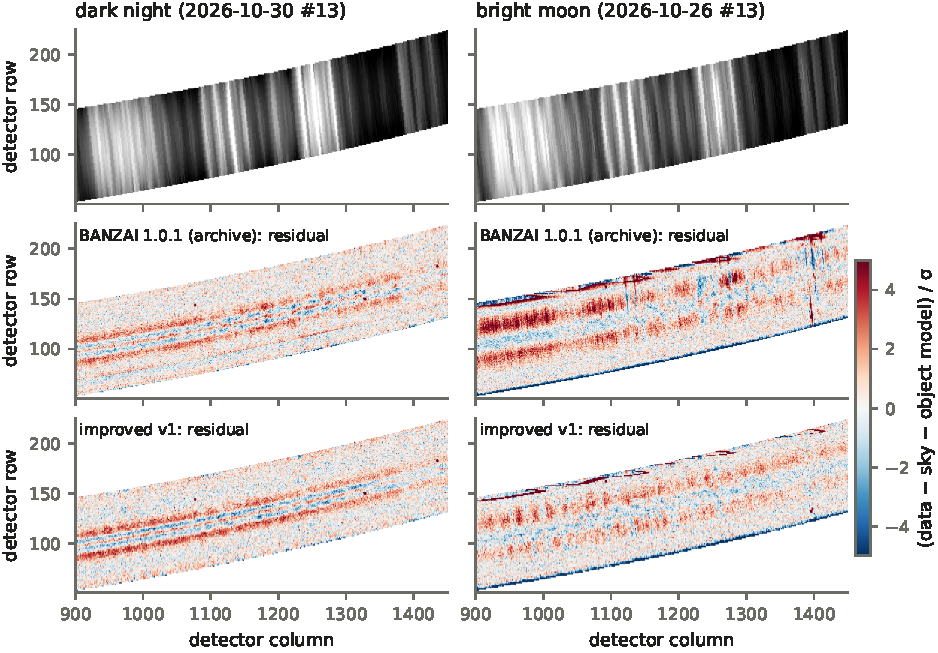
\includegraphics[width=\textwidth]{figures/fig_residuals.pdf}
\caption{Red order at $\approx7600$--9300\,\AA. Top: new sky model. Middle and bottom: normalised residuals (data $-$
sky $-$ profile $\times$ extracted flux)$/\sigma$ of the archive products and of this work, for a dark and a bright-moon
frame.}
\label{fig:residuals}
\end{figure}


The pixel-to-pixel scatter of the extractions agrees with the propagated uncertainties (ratio 0.8--1.2 in both
orders, before and after), so the extraction noise is photon-limited; the red order has the higher signal-to-noise
ratio (93--116 per 1-pixel bin at 4700--6800\,\AA{} against 39--76 in the blue). The ``noise'' of the red order in
the archive products was produced by the fringe correction and the sensitivity function, not by the extraction.
Optimal and fixed-aperture extractions perform alike on the small-scale metrics; the fixed aperture gives a more
consistent red/blue [O\,{\sc iii}] ratio (\FRBBox{} against \FRBOpt{} per cent), as expected for an extended
narrow-line region.

